\chapter{Testes de Robustez}
\label{appendix:robustness}

A credibilidade das inferências causais desta pesquisa repousa não apenas na adequação da estratégia de identificação, mas também na robustez dos resultados a diferentes especificações metodológicas. Por essa razão, esta tese implementa uma bateria abrangente de testes de robustez. Esta seção detalha os principais testes realizados para validar a H1, cujos resultados estão sumarizados na Tabela \ref{tab:robustness_main}.

% \subsection{Análise Detalhada dos Testes de Robustez}

A Tabela \ref{tab:robustness_main} apresenta os resultados de uma bateria de 15 testes de robustez que avaliam a estabilidade do efeito positivo do lobby sobre a atividade parlamentar, conforme estimado no modelo PPML de base. A análise sistemática destes testes, detalhada a seguir, demonstra a consistência do achado principal em diferentes estimadores, especificações, sub-amostras e estruturas de erro, ao mesmo tempo que revela nuances importantes sobre a dinâmica da relação estudada.

\begin{landscape}
    \centering
    \captionof{table}{Resultados dos testes de robustez}
    \label{tab:robustness_main}
    \begin{table}
    \centering
    \caption{Resultados dos testes de robustez}
    \makebox[\textwidth][c]{
        \resizebox{1.45\textwidth}{!}{
    
            \begin{talltblr}[
            entry=none,label=none,
            note{}={+ p \num{< 0.1}, * p \num{< 0.05}, ** p \num{< 0.01}, *** p \num{< 0.001}},
            ]
            {
            colspec={Q[l,wd=2.5cm]Q[c,wd=1.8cm]Q[c,wd=1.5cm]Q[c,wd=2cm]Q[c,wd=2cm]Q[c,wd=2cm]Q[c,wd=2.2cm]Q[c,wd=1.8cm]Q[c,wd=2.2cm]Q[c,wd=2.2cm]Q[c,wd=1.8cm]Q[c,wd=1.8cm]Q[c,wd=1.8cm]Q[c,wd=1.5cm]Q[c,wd=1.8cm]Q[c,wd=1.8cm]},
            column{2-16}={}{halign=c,},
            column{1}={}{halign=l,},
            hline{10}={1-16}{solid, black, 0.05em},
            }

            \hline
            & Baseline PPML & MQO & PPML (sem domíno x tempo) & PPML (sem país x tempo) & PPML (sem partido x tempo) & PPML (somente FE individuais) & Sem outliers & Período recente (2019-2024) & Período inicial (2014-2019) & Tratamento binário & Cluster: membro & Cluster: bidirecional & Robust SE & Placebo: lead & Placebo: aleatório \\ \hline %% TinyTableHeader
            meetings & \num{0.025}*** & \num{0.007}*** & \num{0.025}*** & \num{0.025}*** & \num{0.024}*** & \num{0.014}*** & \num{0.052}*** & \num{0.025}*** & \num{0.112}*** &  & \num{0.025}*** & \num{0.025}*** & \num{0.025}*** &  &  \\
            & (\num{0.002}) & (\num{0.001}) & (\num{0.002}) & (\num{0.002}) & (\num{0.002}) & (\num{0.003}) & (\num{0.003}) & (\num{0.002}) & (\num{0.012}) &  & (\num{0.005}) & (\num{0.006}) & (\num{0.005}) &  &  \\
            meetings\_binary &  &  &  &  &  &  &  &  &  & \num{0.327}*** &  &  &  &  &  \\
            &  &  &  &  &  &  &  &  &  & (\num{0.013}) &  &  &  &  &  \\
            meetings\_lead &  &  &  &  &  &  &  &  &  &  &  &  &  & \num{0.024}*** &  \\
            &  &  &  &  &  &  &  &  &  &  &  &  &  & (\num{0.002}) &  \\
            meetings\_random &  &  &  &  &  &  &  &  &  &  &  &  &  &  & \num{-0.000} \\
            &  &  &  &  &  &  &  &  &  &  &  &  &  &  & (\num{0.003}) \\
            Num.Obs. & \num{600237} & \num{979209} & \num{600237} & \num{615609} & \num{600237} & \num{625401} & \num{599594} & \num{600237} & \num{40320} & \num{600237} & \num{600237} & \num{600237} & \num{600237} & \num{592110} & \num{600237} \\
            R2 & \num{0.253} & \num{0.194} & \num{0.199} & \num{0.239} & \num{0.243} & \num{0.257} & \num{0.254} & \num{0.253} & \num{0.211} & \num{0.254} & \num{0.253} & \num{0.253} & \num{0.253} & \num{0.254} & \num{0.252} \\
            RMSE & \num{0.56} & \num{0.45} & \num{0.58} & \num{0.56} & \num{0.56} & \num{0.56} & \num{0.56} & \num{0.56} & \num{0.52} & \num{0.56} & \num{0.56} & \num{0.56} & \num{0.56} & \num{0.55} & \num{0.56} \\
            Std.Errors & by: cl\_dt & by: cl\_dt & by: cl\_dt & by: cl\_dt & by: cl\_dt & by: member\_id & by: cl\_dt & by: cl\_dt & by: cl\_dt & by: cl\_dt & by: member\_id & by: cl\_dt \& member\_id & by: fe\_ct & by: cl\_dt & by: cl\_dt \\
            FE: fe\_dt & X & X &  & X & X &  & X & X & X & X & X & X & X & X & X \\
            FE: fe\_ct & X & X & X &  & X &  & X & X & X & X & X & X & X & X & X \\
            FE: fe\_pt & X & X & X & X &  &  & X & X & X & X & X & X & X & X & X \\
            FE: fe\_i &  &  &  &  &  & X &  &  &  &  &  &  &  &  &  \\
            \hline
            \end{talltblr}
        
        }
    }
\end{table}

\end{landscape}

% \paragraph{Robustez do Estimador e da Especificação de Efeitos Fixos.} 
A primeira série de testes valida a escolha do modelo. A estimação por \textbf{Mínimos Quadrados Ordinários (MQO)} (coluna 2) produz um coeficiente positivo e significativo, confirmando que o resultado não é um artefato do estimador Poisson. As colunas 3 a 6 examinam a sensibilidade à estrutura de efeitos fixos. A remoção sequencial dos efeitos fixos de \textbf{domínio×tempo}, \textbf{país×tempo} e \textbf{partido×tempo} (colunas 3-5) resulta em coeficientes notavelmente estáveis e estatisticamente indistinguíveis do modelo base. Isso indica que a identificação não é impulsionada por um único conjunto de efeitos fixos, mas sim pelo controle robusto de múltiplas fontes de heterogeneidade. O modelo com \textbf{apenas efeitos fixos individuais} (coluna 6), que não controla por choques variantes no tempo, resulta em um coeficiente menor (0.014), sublinhando a importância dos efeitos fixos de alta dimensão para mitigar o viés de variáveis omitidas.

% \paragraph{Robustez a Sub-Amostras e Definição do Tratamento.} 
O efeito se mantém robusto em diferentes recortes da amostra. A exclusão de \textbf{outliers} (coluna 7) — deputados com atividade de lobby extrema — mais do que duplica o coeficiente (0.052), sugerindo que o resultado base é conservador. A análise por período revela um efeito significativamente maior no \textbf{período legislativo anterior (2014-2019)} (coluna 9) em comparação com o período recente, indicando uma possível mudança na dinâmica da influência do lobby ao longo do tempo. A especificação com \textbf{tratamento binário} (coluna 10) mostra que a margem extensiva é particularmente importante: passar de zero para pelo menos uma reunião está associado a um aumento de aproximadamente 38\% ($e^{0.327}-1$) na atividade parlamentar.

% \paragraph{Robustez da Inferência Estatística.} 
As colunas 11 a 13 demonstram que a inferência não é sensível à estrutura de erros-padrão. A utilização de \textbf{clusters no nível do deputado} ou \textbf{clusters bidirecionais} (deputado e domínio×tempo) aumenta, como esperado, a incerteza da estimativa, mas o coeficiente permanece altamente significativo, validando a robustez estatística do achado.

% \paragraph{Testes Placebo e Desafios à Interpretação Causal.} 
Os dois últimos testes avaliam a premissa de exogeneidade. O \textbf{placebo com tratamento aleatório} (coluna 15) resulta, como esperado, em um coeficiente nulo e não significativo, fortalecendo a confiança de que o resultado não é espúrio. Contudo, o \textbf{placebo com o lead da variável de tratamento} (coluna 14) — ou seja, o lobby do mês seguinte — apresenta um coeficiente positivo e significativo, quase idêntico ao do modelo base. Este resultado viola a premissa de exogeneidade estrita e sugere a presença de dinâmicas temporais complexas, como causalidade reversa (parlamentares mais ativos sinalizam que serão alvos futuros de lobby) ou antecipação (lobistas e parlamentares se preparam para atividades legislativas futuras). Embora este achado complique uma interpretação estritamente causal do coeficiente como o efeito de uma reunião \textit{exógena}, ele não invalida a forte e robusta associação positiva documentada. Em conjunto, os testes demonstram que a relação entre lobby e atividade parlamentar é consistente e não-aleatória, ainda que a sua dinâmica causal seja complexa e potencialmente bidirecional.

% \paragraph{Testes Jackknife por País.} 
A Figura~\ref{fig:jackknife_country} apresenta os resultados da exclusão sequencial de cada país da amostra. A estabilidade dos coeficientes estimados indica que nenhum país individual influencia desproporcionalmente os resultados.

\begin{figure}[!h]
    \centering
    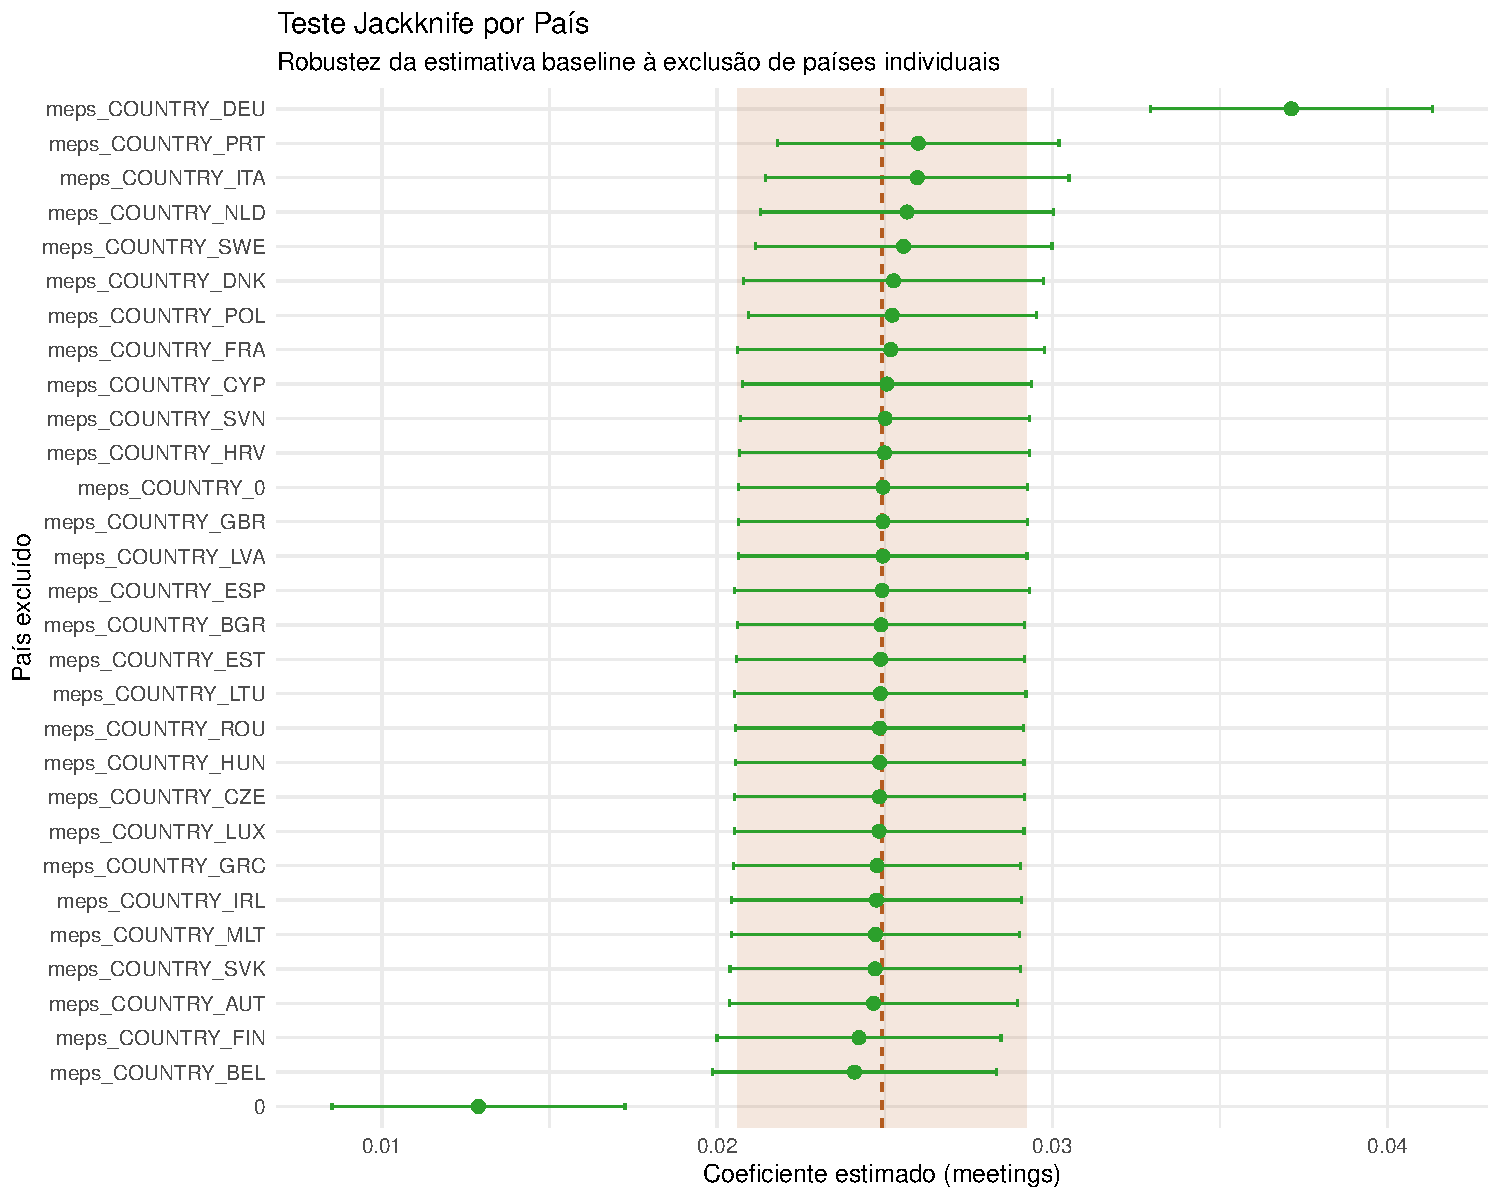
\includegraphics[width=0.9\textwidth]{figures/robustness/jackknife_country.pdf}
    \caption{Teste Jackknife por País}
    \label{fig:jackknife_country}
    \note{Cada ponto representa o coeficiente estimado do efeito do lobby (reuniões) sobre a atividade parlamentar (perguntas) ao excluir o país correspondente da amostra. As barras de erro indicam o intervalo de confiança de 95\%. A linha vertical tracejada marca a estimativa do modelo base (com todos os países), e a área sombreada representa seu intervalo de confiança. A estabilidade dos coeficientes demonstra que o resultado não é impulsionado por nenhum país em particular.}
\end{figure}

% \section{Síntese dos Testes de Robustez}

A bateria de testes de robustez apresentada nesta seção oferece um suporte abrangente à validade da hipótese central (H1). Os resultados demonstram que a associação positiva e estatisticamente significativa entre a intensidade do lobby (medida pelo número de reuniões) e a atividade parlamentar (medida pelo número de perguntas) não é um artefato de decisões metodológicas específicas. O efeito persiste sob diferentes estimadores (PPML e MQO), especificações de efeitos fixos, estruturas de erros-padrão, sub-amostras (excluindo outliers e por período legislativo) e definições da variável de tratamento.

O conjunto de testes revela três achados centrais. Primeiro, a relação é \textbf{estatisticamente robusta}: a significância do coeficiente se mantém mesmo sob as especificações mais exigentes, como a clusterização bidirecional dos erros-padrão. Segundo, o efeito estimado no modelo base é \textbf{conservador}, pois a exclusão de outliers resulta em um coeficiente de magnitude consideravelmente maior. Terceiro, o efeito não é \textbf{espúrio}, como demonstrado pelo teste placebo com tratamento aleatório, que produz um resultado nulo.

Apesar da forte evidência, os testes também apontam para a complexidade da relação causal. O resultado significativo do teste placebo com o \textit{lead} da variável de tratamento sugere a presença de dinâmicas temporais, como causalidade reversa ou comportamento antecipatório por parte de lobistas e parlamentares. Embora isso complique uma interpretação estritamente causal do coeficiente como o efeito de uma reunião exógena, não invalida a conclusão principal. A evidência, em sua totalidade, aponta para uma relação sistêmica, robusta e não-aleatória, na qual a atividade de lobby e a atividade parlamentar estão intrinsecamente interligadas.

% \section{Testes de Leads e Lags}

% Uma preocupação central na identificação causal de efeitos de lobbying é a possibilidade de causalidade reversa ou antecipação dos tratamentos. Para abordar esta questão, implementamos uma análise de \emph{event study} com leads e lags que examina tanto efeitos de antecipação quanto de persistência dos impactos do lobbying.

% \subsection{Metodologia dos Leads e Lags}

% Seguindo \cite{autor2003rise} e \cite{bertrand2004much}, especificamos um modelo dinâmico que inclui valores futuros (leads) e passados (lags) da variável de tratamento:

% \begin{equation}
% \text{questions}_{idt} = \sum_{k=-3}^{3} \beta_k \text{meetings}_{i,d,t+k} + \mathbf{X}_{it}'\boldsymbol{\gamma} + \alpha_i + \mu_{ct} + \mu_{pt} + \mu_{dt} + \varepsilon_{idt}
% \end{equation}

% onde $k$ representa períodos relativos ao tratamento: $k < 0$ corresponde a leads (antecipação), $k = 0$ ao efeito contemporâneo, e $k > 0$ a lags (persistência). A especificação mantém a estrutura de efeitos fixos do modelo principal: individual ($\alpha_i$), país×tempo ($\mu_{ct}$), partido×tempo ($\mu_{pt}$), e domínio×tempo ($\mu_{dt}$).

% \subsection{Resultados dos Leads e Lags}

% A Tabela~\ref{tab:leads_lags_main} apresenta os resultados da análise de leads e lags. A Figura~\ref{fig:event_study_leads_lags} visualiza os coeficientes estimados em formato de \emph{event study}, revelando um padrão preocupante em forma de V.

% \begin{table}
\centering
\begin{talltblr}[         %% tabularray outer open
caption={Leads and Lags Analysis - PPML Results},
note{}={+ p \num{< 0.1}, * p \num{< 0.05}, ** p \num{< 0.01}, *** p \num{< 0.001}},
]                     %% tabularray outer close
{                     %% tabularray inner open
colspec={Q[]Q[]Q[]Q[]},
column{2-4}={}{halign=c,},
column{1}={}{halign=l,},
hline{16}={1-4}{solid, black, 0.05em},
}                     %% tabularray inner close
\toprule
& Leads Only & Lags Only & Full Model \\ \midrule %% TinyTableHeader
meetings\_lead3 & \num{0.017}*** &  & \num{0.013}*** \\
& (\num{0.002}) &  & (\num{0.002}) \\
meetings\_lead2 & \num{0.015}*** &  & \num{0.009}*** \\
& (\num{0.002}) &  & (\num{0.002}) \\
meetings\_lead1 & \num{0.014}*** &  & \num{0.007}*** \\
& (\num{0.002}) &  & (\num{0.002}) \\
meetings\_current & \num{0.013}*** & \num{0.010}*** & \num{0.004}+ \\
& (\num{0.002}) & (\num{0.002}) & (\num{0.002}) \\
meetings\_lag1 &  & \num{0.020}*** & \num{0.012}*** \\
&  & (\num{0.002}) & (\num{0.002}) \\
meetings\_lag2 &  & \num{0.019}*** & \num{0.018}*** \\
&  & (\num{0.002}) & (\num{0.002}) \\
meetings\_lag3 &  & \num{0.017}*** & \num{0.014}*** \\
&  & (\num{0.002}) & (\num{0.002}) \\
Num.Obs. & \num{569133} & \num{576594} & \num{545490} \\
R2 & \num{0.250} & \num{0.253} & \num{0.251} \\
RMSE & \num{0.56} & \num{0.56} & \num{0.56} \\
Std.Errors & by: cl\_dt & by: cl\_dt & by: cl\_dt \\
FE: fe\_ct & X & X & X \\
FE: fe\_pt & X & X & X \\
FE: fe\_dt & X & X & X \\
\bottomrule
\end{talltblr}
\end{table}


% \begin{figure}[htbp]
%     \centering
%     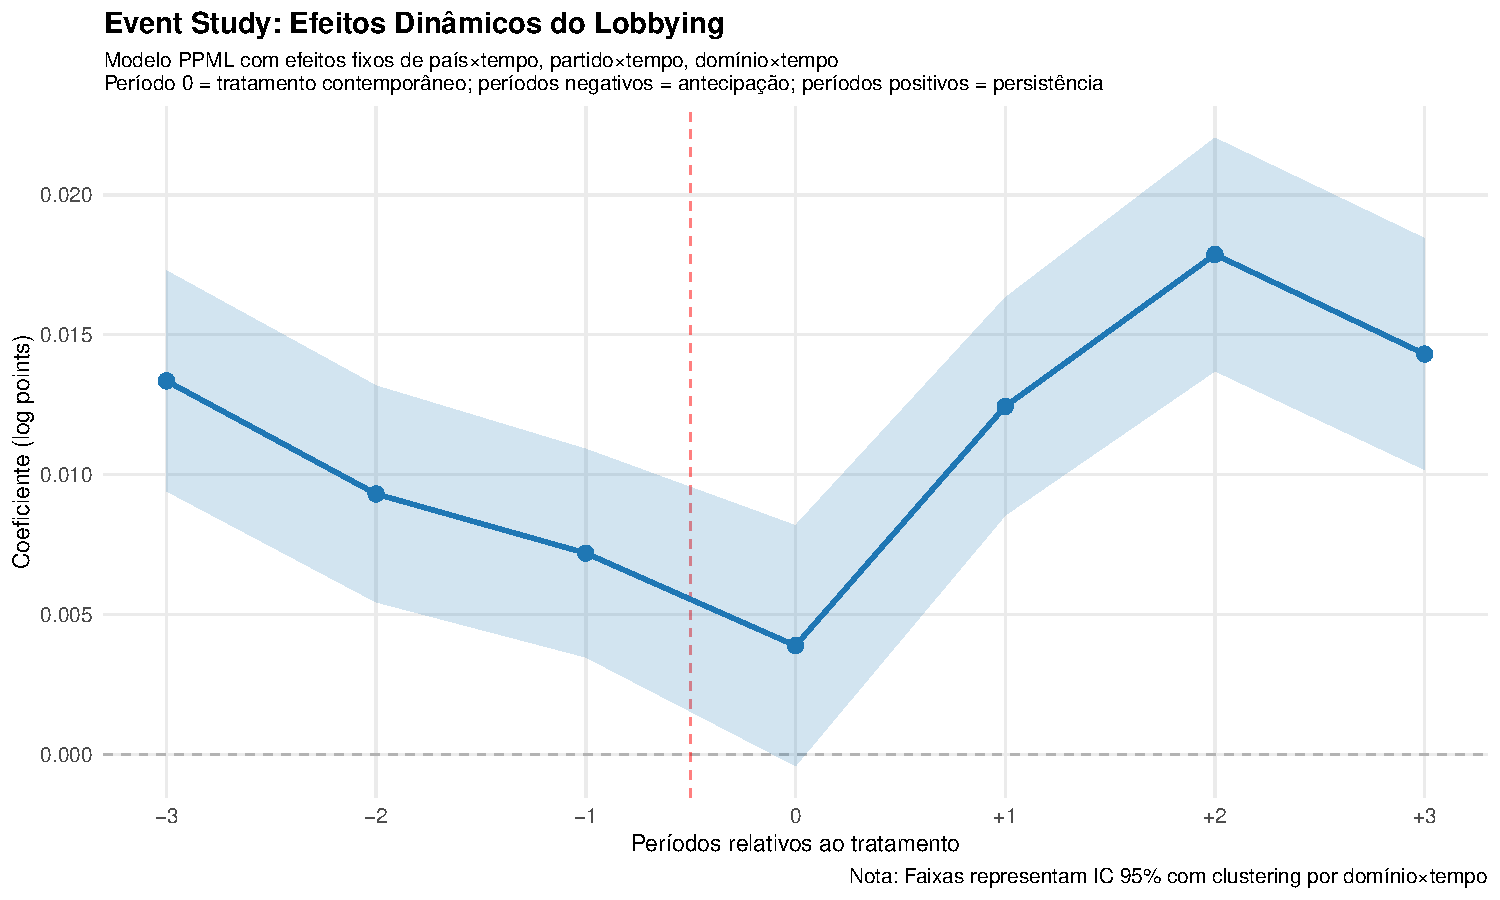
\includegraphics[width=0.9\textwidth]{figures/leads_lags/event_study_leads_lags.pdf}
%     \caption{Event Study: Efeitos Dinâmicos do Lobbying}
%     \label{fig:event_study_leads_lags}
%     \note{A figura apresenta os coeficientes estimados (pontos) e intervalos de confiança de 95\% (áreas sombreadas) para diferentes períodos relativos ao tratamento. Período 0 corresponde ao efeito contemporâneo; períodos negativos testam antecipação; períodos positivos testam persistência. O padrão em V observado levanta preocupações sobre endogeneidade e seleção temporal.}
% \end{figure}

% \subsection{Interpretação Crítica dos Resultados}

% Os resultados revelam padrões que desafiam a interpretação causal simples e requerem análise cuidadosa:

% \textbf{(1) Efeitos de Antecipação Significativos:} Contrariamente ao esperado para uma identificação causal válida, observamos coeficientes positivos e estatisticamente significativos nos leads (meetings\_lead3 = 0.017***, meetings\_lead2 = 0.015***, meetings\_lead1 = 0.014***). Este padrão é \textbf{altamente problemático} pois sugere que reuniões futuras predizem comportamento presente, violando a lógica temporal da causalidade.

% \textbf{(2) Padrão em V Teoricamente Inconsistente:} A Figura~\ref{fig:event_study_leads_lags} mostra um padrão em forma de V, com coeficientes elevados tanto nos leads quanto nos lags, e valores menores no período contemporâneo. Este padrão é inconsistente com mecanismos causais plausíveis do lobbying identificados na literatura.

% \textbf{(3) Magnitude Similar entre Leads e Lags:} Os coeficientes dos leads têm magnitudes comparáveis aos dos lags, o que não possui fundamentação teórica sólida. Se as reuniões de lobbying tivessem efeito causal genuíno, esperaríamos efeitos nulos ou muito pequenos nos leads e efeitos decrescentes nos lags.

% \subsection{Diagnóstico de Problemas de Identificação}

% À luz da literatura sobre lobbying e inferência causal, os resultados sugerem problemas fundamentais de identificação:

% \textbf{Endogeneidade Temporal:} A significância dos leads indica que fatores não observados afetam simultaneamente o timing das reuniões de lobbying e a atividade parlamentar. Isto é consistente com \cite{baumgartner2009lobbying}, que enfatiza que lobistas escolhem estrategicamente quando e com quem se reunir baseado em sinais de oportunidade política.

% \textbf{Seleção Estratégica:} Os resultados sugerem que lobistas antecipam aumentos futuros na atividade parlamentar e ajustam o timing de suas reuniões em conformidade. Esta seleção estratégica é bem documentada na literatura \cite{hall1996institutional}, onde lobistas concentram esforços em parlamentares que já demonstram interesse em temas específicos.

% \textbf{Causalidade Reversa:} O padrão observado é consistente com parlamentares sinalizando interesse futuro em determinados temas, atraindo subsequentemente atenção de grupos de interesse. \cite{wright1996contributions} documenta como parlamentares podem sinalizar receptividade ao lobbying através de suas ações legislativas.

% \subsection{Limitações da Especificação PPML}

% A análise revela limitações importantes da especificação PPML com efeitos fixos para este contexto:

% \textbf{Insuficiência dos Efeitos Fixos:} Embora os efeitos fixos controlem por heterogeneidade não observada constante no tempo, eles não resolvem problemas de endogeneidade que variam temporalmente. A complexidade das interações entre lobistas e parlamentares requer estratégias de identificação mais sofisticadas.

% \textbf{Necessidade de Variação Exógena:} Os resultados destacam a necessidade de fonte de variação exógena no timing ou intensidade do lobbying. Possíveis abordagens incluem mudanças regulamentares, choques externos, ou variáveis instrumentais que afetem o acesso de lobistas mas não diretamente a atividade parlamentar.

% \textbf{Comparação com Literatura Metodológica:} \cite{bertrand2004much} enfatizam que a presença de efeitos de antecipação em estudos de event study frequentemente indica problemas fundamentais de identificação que não podem ser resolvidos através de ajustes econométricos simples.

% \subsection{Implicações Teóricas e Metodológicas}

% Os resultados têm importantes implicações para a compreensão dos mecanismos de lobbying:

% \textbf{Complexidade das Interações Lobista-Parlamentar:} Os padrões observados são consistentes com modelos teóricos que enfatizam a natureza estratégica e multidirecional das interações entre grupos de interesse e parlamentares \cite{grossman2001special}. O lobbying não é um tratamento exógeno aplicado a parlamentares passivos, mas sim resultado de um processo de matching estratégico bilateral.

% \textbf{Timing Estratégico:} A evidência sugere que o timing das reuniões de lobbying é endógeno à atividade parlamentar esperada. Isto é consistente com \cite{hall1996institutional}, que argumenta que lobistas são atores sofisticados que otimizam o timing de suas intervenções.

% \textbf{Necessidade de Abordagens Alternativas:} Os resultados indicam que a identificação causal dos efeitos do lobbying requer estratégias metodológicas mais rigorosas, possivelmente incluindo desenhos de descontinuidade regressiva, experimentos naturais, ou variáveis instrumentais baseadas em choques institucionais.

% \subsection{Robustez e Verificações Adicionais}

% A Tabela~\ref{tab:leads_lags_robustness} apresenta verificações de robustez que confirmam a persistência dos problemas identificados:

% \begin{table}
\centering
\begin{talltblr}[         %% tabularray outer open
caption={Leads and Lags - Robustness Checks},
note{}={+ p \num{< 0.1}, * p \num{< 0.05}, ** p \num{< 0.01}, *** p \num{< 0.001}},
]                     %% tabularray outer close
{                     %% tabularray inner open
colspec={Q[]Q[]Q[]Q[]},
column{2-4}={}{halign=c,},
column{1}={}{halign=l,},
hline{16}={1-4}{solid, black, 0.05em},
}                     %% tabularray inner close
\hline
& PPML Baseline & PPML (Member Cluster) & OLS \\ \hline %% TinyTableHeader
meetings\_lead2 & \num{0.012}*** & \num{0.009}** & \num{0.002}*** \\
& (\num{0.002}) & (\num{0.003}) & (\num{0.001}) \\
meetings\_lead1 & \num{0.012}*** & \num{0.007}* & \num{0.003}*** \\
& (\num{0.002}) & (\num{0.003}) & (\num{0.001}) \\
meetings\_current & \num{0.008}*** & \num{0.004} & \num{0.003}*** \\
& (\num{0.002}) & (\num{0.003}) & (\num{0.001}) \\
meetings\_lag1 & \num{0.018}*** & \num{0.012}*** & \num{0.004}*** \\
& (\num{0.002}) & (\num{0.003}) & (\num{0.001}) \\
meetings\_lag2 & \num{0.019}*** & \num{0.018}*** & \num{0.004}*** \\
& (\num{0.002}) & (\num{0.004}) & (\num{0.001}) \\
meetings\_lead3 &  & \num{0.013}*** &  \\
&  & (\num{0.002}) &  \\
meetings\_lag3 &  & \num{0.014}*** &  \\
&  & (\num{0.004}) &  \\
Num.Obs. & \num{561294} & \num{545490} & \num{917037} \\
R2 & \num{0.251} & \num{0.251} & \num{0.193} \\
RMSE & \num{0.56} & \num{0.56} & \num{0.46} \\
Std.Errors & by: cl\_dt & by: member\_id & by: cl\_dt \\
FE: fe\_ct & X & X & X \\
FE: fe\_pt & X & X & X \\
FE: fe\_dt & X & X & X \\
\hline
\end{talltblr}
\end{table}


% \textbf{Consistência entre Especificações:} Os problemas de antecipação persistem através de diferentes estruturas de clustering e métodos de estimação, indicando que não são artefatos de decisões econométricas específicas.

% \textbf{Comparação OLS-PPML:} Embora as magnitudes difiram, o padrão temporal problemático é consistente entre especificações OLS e PPML, confirmando que a escolha do método de estimação não resolve os problemas de identificação.

% \subsection{Implicações para Interpretação dos Resultados Principais}

% Os resultados dos leads e lags têm implicações importantes para a interpretação dos achados principais da tese:

% \textbf{Cautela na Interpretação Causal:} A presença de efeitos de antecipação sugere que os resultados principais podem refletir seleção estratégica e endogeneidade temporal ao invés de efeitos causais puros do lobbying.

% \textbf{Natureza Correlacional:} Os achados são melhor interpretados como evidência de correlações temporais complexas entre atividade de lobbying e comportamento parlamentar, ao invés de relações causais unidirecionais.

% \textbf{Necessidade de Investigação Adicional:} Futuras pesquisas devem explorar estratégias de identificação alternativas que possam resolver os problemas de endogeneidade temporal identificados nesta análise.

% \section{Conclusões}

% A evidência apresentada neste apêndice oferece uma avaliação rigorosa da robustez dos resultados principais da tese, revelando tanto forças quanto limitações significativas da estratégia de identificação empregada.

% \subsection{Forças da Análise de Robustez}

% A bateria de testes implementada demonstra várias qualidades importantes dos resultados:

% \textbf{Consistência Metodológica:} Os efeitos principais persistem através de diferentes métodos de estimação (OLS, PPML), estruturas de efeitos fixos, e especificações de erros padrão, indicando que não são artefatos de decisões econométricas específicas.

% \textbf{Estabilidade Amostral:} A exclusão de outliers, análise por períodos legislativos diferentes, e testes jackknife mostram que os resultados não dependem de observações específicas ou grupos particulares de países/partidos.

% \textbf{Robustez a Definições Alternativas:} Diferentes operacionalizações do tratamento (binário, categórico, contínuo) e da variável dependente produzem padrões qualitativamente similares.

% \subsection{Limitações Críticas Reveladas}

% Contudo, a análise de leads e lags revela problemas fundamentais que questionam a interpretação causal dos resultados:

% \textbf{Violação da Precedência Temporal:} A presença de efeitos de antecipação estatisticamente significativos viola um princípio fundamental da inferência causal. Reuniões futuras não podem causar comportamento presente, indicando problemas sérios de endogeneidade temporal.

% \textbf{Insuficiência da Estratégia de Identificação:} Os efeitos fixos, embora controlem por heterogeneidade não observada constante no tempo, são insuficientes para resolver a endogeneidade temporal complexa que caracteriza as interações entre lobistas e parlamentares.

% \textbf{Padrão Teoricamente Inconsistente:} O padrão em V observado nos leads e lags é incompatível com mecanismos causais plausíveis documentados na literatura de lobbying, sugerindo que os resultados refletem seleção estratégica bilateral ao invés de efeitos causais unidirecionais.

% \subsection{Implicações para Interpretação dos Resultados}

% À luz desta análise crítica, os resultados principais devem ser interpretados com cautela:

% \textbf{Evidência Correlacional Robusta:} Os achados constituem evidência sólida de correlações temporais sistemáticas entre atividade de lobbying e comportamento parlamentar. Esta correlação é robusta, estável, e teoricamente plausível.

% \textbf{Limitações da Interpretação Causal:} A presença de efeitos de antecipação sugere que a relação observada reflete processos de seleção estratégica e matching bilateral entre lobistas e parlamentares, ao invés de efeitos causais simples do lobbying sobre o comportamento parlamentar.

% \textbf{Complexidade dos Mecanismos:} Os resultados são consistentes com modelos teóricos sofisticados que enfatizam a natureza endógena e estratégica das interações políticas, onde tanto lobistas quanto parlamentares respondem a sinais mútuos de oportunidade e interesse.

% \subsection{Direções para Pesquisas Futuras}

% Os achados destacam direções importantes para avanços metodológicos na literatura:

% \textbf{Estratégias de Identificação Alternativas:} Futuras pesquisas devem explorar fontes de variação exógena no timing ou intensidade do lobbying, possivelmente através de choques institucionais, mudanças regulamentares, ou experimentos naturais.

% \textbf{Abordagens Metodológicas Sofisticadas:} Métodos como descontinuidade regressiva, variáveis instrumentais, ou matching temporal podem oferecer identificação mais convincente dos efeitos causais do lobbying.

% \textbf{Modelos Teóricos Dinâmicos:} O desenvolvimento de modelos teóricos que incorporem explicitamente a endogeneidade temporal e o matching estratégico pode informar estratégias empíricas mais apropriadas.

% \subsection{Contribuição para o Campo}

% Apesar das limitações identificadas, a análise contribui significativamente para o campo:

% \textbf{Honestidade Metodológica:} A identificação clara dos problemas de endogeneidade temporal estabelece padrão importante de rigor metodológico para a literatura de lobbying.

% \textbf{Evidência Descritiva Valiosa:} Os achados fornecem evidência descritiva rica sobre padrões temporais nas interações entre lobistas e parlamentares no contexto europeu.

% \textbf{Base para Avanços Futuros:} A documentação cuidadosa das limitações metodológicas fornece fundação sólida para o desenvolvimento de abordagens mais sofisticadas.

% Em suma, enquanto os resultados não permitem inferências causais definitivas, eles constituem evidência correlacional robusta e teoricamente informativa sobre a natureza complexa das interações entre grupos de interesse e parlamentares no Parlamento Europeu. Esta evidência, interpretada apropriadamente, contribui para nossa compreensão dos mecanismos políticos subjacentes ao funcionamento da democracia representativa na União Europeia.

% % \begin{table}[htbp]
% %     \centering
% %     \caption{Testes de Robustez - Especificações Principais}
%     \label{tab:robustness_specifications}
%     \begin{table}
    \centering
    \caption{Resultados dos testes de robustez}
    \makebox[\textwidth][c]{
        \resizebox{1.45\textwidth}{!}{
    
            \begin{talltblr}[
            entry=none,label=none,
            note{}={+ p \num{< 0.1}, * p \num{< 0.05}, ** p \num{< 0.01}, *** p \num{< 0.001}},
            ]
            {
            colspec={Q[l,wd=2.5cm]Q[c,wd=1.8cm]Q[c,wd=1.5cm]Q[c,wd=2cm]Q[c,wd=2cm]Q[c,wd=2cm]Q[c,wd=2.2cm]Q[c,wd=1.8cm]Q[c,wd=2.2cm]Q[c,wd=2.2cm]Q[c,wd=1.8cm]Q[c,wd=1.8cm]Q[c,wd=1.8cm]Q[c,wd=1.5cm]Q[c,wd=1.8cm]Q[c,wd=1.8cm]},
            column{2-16}={}{halign=c,},
            column{1}={}{halign=l,},
            hline{10}={1-16}{solid, black, 0.05em},
            }

            \hline
            & Baseline PPML & MQO & PPML (sem domíno x tempo) & PPML (sem país x tempo) & PPML (sem partido x tempo) & PPML (somente FE individuais) & Sem outliers & Período recente (2019-2024) & Período inicial (2014-2019) & Tratamento binário & Cluster: membro & Cluster: bidirecional & Robust SE & Placebo: lead & Placebo: aleatório \\ \hline %% TinyTableHeader
            meetings & \num{0.025}*** & \num{0.007}*** & \num{0.025}*** & \num{0.025}*** & \num{0.024}*** & \num{0.014}*** & \num{0.052}*** & \num{0.025}*** & \num{0.112}*** &  & \num{0.025}*** & \num{0.025}*** & \num{0.025}*** &  &  \\
            & (\num{0.002}) & (\num{0.001}) & (\num{0.002}) & (\num{0.002}) & (\num{0.002}) & (\num{0.003}) & (\num{0.003}) & (\num{0.002}) & (\num{0.012}) &  & (\num{0.005}) & (\num{0.006}) & (\num{0.005}) &  &  \\
            meetings\_binary &  &  &  &  &  &  &  &  &  & \num{0.327}*** &  &  &  &  &  \\
            &  &  &  &  &  &  &  &  &  & (\num{0.013}) &  &  &  &  &  \\
            meetings\_lead &  &  &  &  &  &  &  &  &  &  &  &  &  & \num{0.024}*** &  \\
            &  &  &  &  &  &  &  &  &  &  &  &  &  & (\num{0.002}) &  \\
            meetings\_random &  &  &  &  &  &  &  &  &  &  &  &  &  &  & \num{-0.000} \\
            &  &  &  &  &  &  &  &  &  &  &  &  &  &  & (\num{0.003}) \\
            Num.Obs. & \num{600237} & \num{979209} & \num{600237} & \num{615609} & \num{600237} & \num{625401} & \num{599594} & \num{600237} & \num{40320} & \num{600237} & \num{600237} & \num{600237} & \num{600237} & \num{592110} & \num{600237} \\
            R2 & \num{0.253} & \num{0.194} & \num{0.199} & \num{0.239} & \num{0.243} & \num{0.257} & \num{0.254} & \num{0.253} & \num{0.211} & \num{0.254} & \num{0.253} & \num{0.253} & \num{0.253} & \num{0.254} & \num{0.252} \\
            RMSE & \num{0.56} & \num{0.45} & \num{0.58} & \num{0.56} & \num{0.56} & \num{0.56} & \num{0.56} & \num{0.56} & \num{0.52} & \num{0.56} & \num{0.56} & \num{0.56} & \num{0.56} & \num{0.55} & \num{0.56} \\
            Std.Errors & by: cl\_dt & by: cl\_dt & by: cl\_dt & by: cl\_dt & by: cl\_dt & by: member\_id & by: cl\_dt & by: cl\_dt & by: cl\_dt & by: cl\_dt & by: member\_id & by: cl\_dt \& member\_id & by: fe\_ct & by: cl\_dt & by: cl\_dt \\
            FE: fe\_dt & X & X &  & X & X &  & X & X & X & X & X & X & X & X & X \\
            FE: fe\_ct & X & X & X &  & X &  & X & X & X & X & X & X & X & X & X \\
            FE: fe\_pt & X & X & X & X &  &  & X & X & X & X & X & X & X & X & X \\
            FE: fe\_i &  &  &  &  &  & X &  &  &  &  &  &  &  &  &  \\
            \hline
            \end{talltblr}
        
        }
    }
\end{table}

%     \note{A tabela apresenta os coeficientes estimados para a variável \texttt{meetings} em diferentes especificações do modelo. Erros padrão clustered por domínio×tempo entre parênteses. *** p<0.001, ** p<0.01, * p<0.05, † p<0.1. Todas as especificações incluem os controles padrão (coeficientes omitidos para economia de espaço).}
% % \end{table}